% !TeX root = surprises.tex

\chapter{La brújula se hunde}\label{c.collapse}

%%%%%%%%%%%%%%%%%%%%%%%%%%%%%%%%%%%%%%%%%%%%%%%%%%%%%%%%%%%%%%%

Una brújula moderna es un compás fijo: la distancia entre las dos patas puede fijarse de modo que es posible copiar un segmento de línea o un círculo de una posición a otra (Fig.~\ref{fig.fixed-compass}). Euclides utilizó un \emph{brújula de colapso} cuando no se puede mantener una distancia fija (Fig.~\ref{fig.collapsing-compass}). Los profesores suelen utilizar un compás colapsable consistente en un rotulador atado a una cuerda que se utiliza para construir un círculo en una pizarra. Es imposible mantener una longitud fija cuando se retira el compás de la pizarra. 

\begin{figure}[htb]
\begin{minipage}{.45\textwidth}
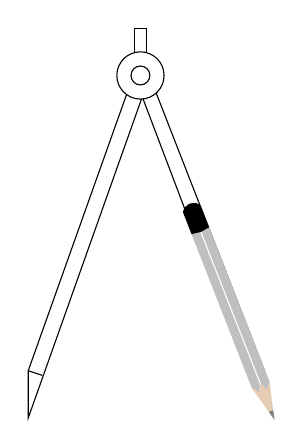
\begin{tikzpicture}
\begin{scope}[rotate=0,transform shape,scale=3]
\draw (2.95,3.7) rectangle (3,3.95);
\draw (2.92,3.68) -- (2.5,2.5) -- (2.5,2.3) -- (2.99,3.68);
\draw (3.5,2.5) -- (3.43,2.48) -- (2.975,3.68);
\draw (3.04,3.68) -- (3.5,2.5);
\draw (2.5,2.5) -- (2.56,2.48);
\draw[fill=white] (2.975,3.75) circle (0.1cm);
\draw (2.975,3.75) circle (0.04cm);
\end{scope}
\begin{scope}[xshift=10.34cm,yshift=7.28cm,rotate=21.4,scale=.6]          
\fill[gray!50] (0,4) -- (0.4,4) -- (0.4,0) --
               (0.3,-0.15) -- (0.2,0) -- (0.1,-0.14) --
               (0,0) -- cycle;
\draw[color=white] (0.2,4) -- (0.2,0);
\fill[black] (0,3.5) -- (0.2,3.47) -- (0.4,3.5) --
             (0.4,4) arc(30:150:0.23cm);
\fill[brown!40] (0,0) -- (0.2,-0.8)
    node[coordinate,pos=0.75](a){} -- 
    (0.4,0)node[coordinate,pos=0.25](b){} -- 
    (0.3,-0.15) -- (0.2,0) -- (0.1,-0.14) -- cycle;
\fill[gray] (a) -- (0.2,-0.8) -- (b) -- cycle;
\end{scope}
\end{tikzpicture}
\caption{Una brújula fija. Una pata tiene una aguja que se coloca en el centro del círculo. Un lápiz fijado a la otra pata sirve para dibujar el círculo. Las patas están unidas por una bisagra hermética, de modo que la distancia entre las patas (el radio del círculo) se mantiene incluso cuando el compás se levanta del papel.}\label{fig.fixed-compass}
\end{minipage}
\hfill
\begin{minipage}{.45\textwidth}
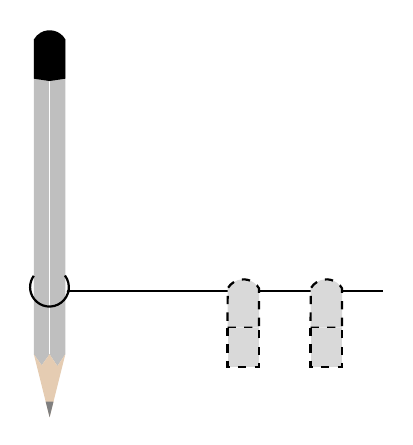
\begin{tikzpicture}[rotate=0,scale=1]          
\fill[gray!50] (0,4) -- (0.4,4) -- (0.4,0) --
               (0.3,-0.15) -- (0.2,0) -- (0.1,-0.14) --
               (0,0) -- cycle;
\draw[color=white] (0.2,4) -- (0.2,0);
\fill[black] (0,3.5) -- (0.2,3.47) -- (0.4,3.5) --
             (0.4,4) arc(30:150:0.23cm);
\fill[brown!40] (0,0) -- (0.2,-0.8)
    node[coordinate,pos=0.75](a){} -- 
    (0.4,0) node[coordinate,pos=0.25](b){} -- 
    (0.3,-0.15) -- (0.2,0) -- (0.1,-0.14) -- cycle;
\fill[gray] (a) -- (0.2,-0.8) -- (b) -- cycle;

\draw[thick] (0.395,1) arc (37:-216:7pt);
\coordinate (knot) at (0.44,.8);
\draw[thick] (knot) -- +(4,0);
\fill (knot) circle (.7pt);

\begin{scope}[xshift=100pt,yshift=-90pt]
\draw[dashed,thick,fill=white!70!gray] (0,3.5) -- (0.4,3.5) -- 
      (0.4,4) arc(30:150:0.23cm) -- cycle;
\draw[dashed,thick,fill=white!70!gray] (0,3.5) -- ++(0,-.5) -- ++(.4,0) -- ++(0,.5);
\end{scope}

\begin{scope}[xshift=70pt,yshift=-90pt]
\draw[dashed,thick,fill=white!70!gray] (0,3.5) -- (0.4,3.5) -- 
      (0.4,4) arc(30:150:0.23cm) -- cycle;
\draw[dashed,thick,fill=white!70!gray] (0,3.5) -- ++(0,-.5) -- ++(.4,0) -- ++(0,.5);
\end{scope}
\end{tikzpicture}
\caption{Un compás colapsable. El usuario sujeta un trozo de cuerda en el centro del círculo. El otro extremo de la cuerda se ata a un lápiz y se utiliza para dibujar el círculo. Cuando se levanta el compás del papel, los dedos (punteados) pueden deslizarse fácilmente hasta una nueva posición.}\label{fig.collapsing-compass}
\end{minipage}
\end{figure}

Este capítulo comienza con una discusión sobre la relevancia de estudiar la construcción con regla y compás (Secc.~\ref{s.relevance}).
En el apartado~\ref{s.collapse} se comparan los dos tipos de compás en la construcción más elemental: una mediatriz. En el apartado~\ref{s.collapse-copy} se presenta el método de Euclides para copiar un segmento de recta utilizando un compás de colapso. Esto demuestra que cualquier construcción que se pueda hacer usando un compás fijo se puede realizar usando un compás colapsable. La sección~\ref{s.collapse-copy-incorrect} muestra una prueba de este teorema que parece correcta, pero no funciona para todas las configuraciones de rectas y puntos. Para enfatizar que no hay que fiarse de los diagramas, la sección ~\ref{s.collapse-isoceles} presenta una famosa supuesta prueba de que todos los triángulos son isoceles; la prueba parece correcta, pero no lo es porque se basa en un diagrama incorrecto.

\section{Construcción con regla y compás}\label{s.relevance}

La construcción con regla y compás solía ser el concepto fundamental que se enseñaba en geometría euclidiana. Recientemente, ha caído en desgracia en los programas escolares. Es cierto que el tema tiene poca o ninguna utilidad práctica. Como mostramos en las secciones~\ref{s.neusis}, \ref{s.neusis-doubling}, \ref{s.q}, \ref{s.square-quad}, los griegos sabían cómo realizar construcciones que son imposibles con una regla y un compás utilizando herramientas sólo ligeramente más avanzadas. Hoy en día, mediante métodos numéricos, los ordenadores pueden realizar construcciones con la precisión que se desee.

No obstante, creo que estudiar las construcciones tiene sus ventajas:
\begin{itemize}
\item Es más divertido y desafiante aprender geometría a través de construcciones que simplemente leyendo teoremas y pruebas.
\item Se han logrado avances significativos en matemáticas mediante intentos de encontrar construcciones. El capítulo~\ref{c.heptadecagon} presenta una construcción de Gauss que condujo al álgebra abstracta moderna, en particular, la teoría desarrollada por \'{E}variste Galois.
\item Es algo contraintuitivo y por lo tanto muy interesante que se pueda demostrar que es imposible construir algunos objetos geométricos.
\item Lamentablemente, hay muchas personas que pierden años de su vida intentando realizar construcciones imposibles. Los estudiantes deberían ser conscientes de la inutilidad de tales esfuerzos.
\end{itemize}

\section{Brújulas fijas y brújulas abatibles}\label{s.collapse}

Algunos libros de geometría presentan la construcción de una mediatriz de un segmento de recta construyendo dos circunferencias centradas en los extremos del segmento de recta de forma que los radios sean iguales y mayores que la mitad de la longitud del segmento (Fig.~\ref{f.collapse-perp-bisector-fixed}). Esto sólo se puede hacer con un compás fijo porque después de dibujar el círculo centrado en $A$, la distancia entre las patas del compás tiene que permanecer fija para dibujar el círculo centrado en $B$.

\begin{figure}[t]
\begin{minipage}{.45\textwidth}
\begin{center}
\begin{tikzpicture}[scale=0.5]
\coordinate (A) at (0,0);
\coordinate (B) at (4,0);
\vertex{A};
\vertex{B};
\draw (A) node[below left] {$A$} -- (B) node[below right] {$B$};
\draw[name path=larc] (A) ++(-60:3cm) arc (-60:60:3cm);
\draw[name path=rarc] (B) ++(-120:3cm) arc (-120:-240:3cm);
\path [name intersections={of=larc and rarc,by={b,t}}];
\node[above right,xshift=-2pt,yshift=5pt] at (t) {$C$};
\node[below left,xshift=2pt,yshift=-5pt] at (b) {$D$};
\draw ($ (b) ! 1.2 ! (t)$) -- ($ (t) ! 1.2 ! (b)$);
\end{tikzpicture}
\caption{Construcción de una mediatriz con compás fijo}\label{f.collapse-perp-bisector-fixed}
\end{center}
\end{minipage}
\hfill
\begin{minipage}{.45\textwidth}
\begin{center}
\begin{tikzpicture}[scale=0.5]
\coordinate (A) at (0,0);
\coordinate (B) at (4,0);
\vertex{A};
\vertex{B};
\draw (A) node[below left] {$A$} -- (B) node[below right] {$B$};
\draw[name path=larc] (A) ++(-80:4cm) arc (-80:80:4cm);
\draw[name path=rarc] (B) ++(-100:4cm) arc (-100:-260:4cm);
\path [name intersections={of=larc and rarc,by={b,t}}];
\node[above right,xshift=-2pt,yshift=3pt] at (t) {$C$};
\node[below left,xshift=2pt,yshift=-3pt] at (b) {$D$};
\draw ($ (b) ! 1.2 ! (t)$) -- ($ (t) ! 1.2 ! (b)$);
\end{tikzpicture}
\caption{Construcción de una mediatriz con compás fijo o de colapso}\label{f.collapse-perp-bisector-collapse}
\end{center}
\end{minipage}
\end{figure}

Figura~\ref{f.collapse-perp-bisector-collapse} muestra la construcción de una mediatriz con compás fijo o con compás abatible. Se construyen dos circunferencias: una centrada en $A$ con radio $\overline{AB}$ y otra centrada en $B$ con radio $\overline{BA}$. Esto se puede hacer con un compás de colapso porque (obviamente) $\overline{AB}=\overline{BA}$, por lo que el compás no tiene que ``recordar'' la longitud de $\overline{AB}$ para construir una circunferencia centrada en $B$ con el mismo radio.
La demostración de que la recta construida mostrada en la Fig.~\ref{f.collapse-perp-bisector-fixed} es una mediatriz no es nada elemental porque hay que utilizar conceptos relativamente avanzados como triángulos congruentes. Sin embargo, la prueba de que la construcción de una mediatriz mostrada en la Fig.~\ref{f.collapse-perp-bisector-collapse} es correcta es sencilla y se basa en el hecho de que $\triangle ABC$ es un triángulo equilátero. De hecho, esta es la primera proposición en el \textit{Elementos} de Euclides.
$\overline{AC}=\overline{AB}$ ya que son radios del mismo círculo, análogamente, $\overline{BC}=\overline{BA}$. Tenemos: $\overline{AC}=\overline{AB}=\overline{BA}=\overline{BC}$.

Figura~\ref{f.collapse-equilateral-fixed} muestra que para la construcción con compás fijo, el triángulo será un triángulo isósceles, no necesariamente equilátero (Fig.~\ref{f.collapse-equilateral-collapse}).

\section{Construcción de Euclides para copiar un segmento de recta}\label{s.collapse-copy}

La segunda proposición del \textit{Elementos} de Euclides describe cómo copiar un segmento de recta $\overline{AB}$ dado en un segmento de la misma longitud, uno de cuyos puntos extremos es un punto $C$ dado. Por lo tanto, un compás fijo no añade ninguna capacidad adicional y basta con un compás colapsable, aunque las construcciones son más fáciles con un compás fijo.

\begin{theorem}
Dado un segmento de recta $\overline{AB}$ y un punto $C$, se puede construir un segmento de recta $\overline{CC'}$, uno de cuyos puntos extremos es $C$, utilizando un compás de colapso, tal que $\overline{AB}=\overline{CC'}$ (Fig.~\ref{f.collapse-copying-1}).
\end{theorem}

\begin{figure}[t]
\begin{minipage}{.45\textwidth}
\begin{center}
\begin{tikzpicture}[scale=0.5]
\coordinate (A) at (0,0);
\coordinate (B) at (4,0);
\vertex{A};
\vertex{B};
\draw (A) node[below left] {$A$} -- (B) node[below right] {$B$};
\draw[name path=larc] (A) ++(-60:3cm) arc (-60:60:3cm);
\draw[name path=rarc] (B) ++(-120:3cm) arc (-120:-240:3cm);
\path [name intersections={of=larc and rarc,by={b,t}}];
\vertex{t};
\vertex{b};
\node[above right,xshift=-2pt,yshift=5pt] at (t) {$C$};
\node[below left,xshift=2pt,yshift=-5pt] at (b) {$D$};
\draw (A) -- (t);
\draw (B) -- (t);
\end{tikzpicture}
\caption{Construcción de un triángulo isóceles con compás fijo}\label{f.collapse-equilateral-fixed}
\end{center}
\end{minipage}
\hfill
\begin{minipage}{.45\textwidth}
\begin{center}
\begin{tikzpicture}[scale=0.5]
\coordinate (A) at (0,0);
\coordinate (B) at (4,0);
\draw (A) node[below left] {$A$} -- (B) node[below right] {$B$};
\vertex{A};
\vertex{B};
\draw[name path=larc] (A) ++(-80:4cm) arc (-80:80:4cm);
\draw[name path=rarc] (B) ++(-100:4cm) arc (-100:-260:4cm);
\path [name intersections={of=larc and rarc,by={b,t}}];
\vertex{t};
\vertex{b};
\node[above right,xshift=-2pt,yshift=3pt] at (t) {$C$};
\node[below left,xshift=2pt,yshift=-3pt] at (b) {$D$};
\draw (A) -- (t);
\draw (B) -- (t);
\end{tikzpicture}
\caption{Construcción de un triángulo equilátero con un compás de derrumbe}\label{f.collapse-equilateral-collapse}
\end{center}
\end{minipage}
\end{figure}

\begin{figure}[b]
\begin{minipage}{.45\textwidth}
\begin{center}
\begin{tikzpicture}[scale=0.5]
\coordinate (C) at (0,0);
\coordinate (A) at (3,0);
\draw (A) node[below,xshift=-2pt,yshift=-2pt] {$A$} -- +(40:4) coordinate (B) node[right] {$B$};
\vertex{A};
\vertex{B};
\vertex{C};
\node[below,xshift=2pt,yshift=-2pt] at (C) {$C$};
\draw[thick,dashed] (C) -- +(160:4) coordinate (D) node[below] {$C'$};
\vertex{D};
\end{tikzpicture}
\caption{Copiar el segmento de recta $\overline{AB}$. La orientación de $\overline{CC'}$ no es importante.}\label{f.collapse-copying-1}
\end{center}
\end{minipage}
\hfill
\begin{minipage}{.45\textwidth}
\begin{center}
\begin{tikzpicture}[scale=0.5]
\coordinate (C) at (0,0);
\coordinate (A) at (3,0);
\draw (A) node[below,xshift=-2pt,yshift=-2pt] {$A$} -- +(40:4) coordinate (B) node[right] {$B$};
\vertex{B};
\node[below,xshift=2pt,yshift=-2pt] at (C) {$C$};
\draw (A) -- (C);
\path[name path=larc] (C) ++(-70:2.5cm) arc (-70:70:2.5cm);
\path[name path=rarc] (A) ++(-110:2.5cm) arc (-110:-250:2.5cm);
\path [name intersections={of=larc and rarc,by={d,D}}];
\node[above] at (D) {$D$};
\draw (A) -- (D);
\draw (C) -- (D);
\end{tikzpicture}
\caption{Copiar un segmento de línea con un compás de colapso}\label{f.collapse-copying-2}
\end{center}
\end{minipage}
\end{figure}

\begin{proof}
Construir el segmento de recta $\overline{AC}$. Construir el triángulo equilátero $\triangle ACD$ cuya base es $\overline{AC}$ (Fig.~\ref{f.collapse-copying-2}). Por la primera proposición de Euclides, el triángulo se puede construir utilizando un compás de colapso. Construir la semirrecta que es prolongación de la recta segmento \emph{de $D$ a $A$}, y construir la semirrecta que es prolongación de la recta segmento \emph{de $D$ a $C$} (Fig.~\ref{f.collapse-copying-3}). Construimos la circunferencia centrada en $A$ con radio $\overline{AB}$ y denotamos la intersección de la circunferencia y la semirrecta que prolonga $\overline{DA}$ por $E$ (Fig.~\ref{f.collapse-copying-4}). Construimos la circunferencia centrada en $D$ con radio $\overline{DE}$ y denotamos por $F$ la intersección de la circunferencia y la semirrecta que prolonga $\overline{DC}$ (Fig.~\ref{f.collapse-copying-5}).

\begin{figure}[t]
\begin{minipage}{.45\textwidth}
\begin{center}
\begin{tikzpicture}[scale=0.4]
\coordinate (C) at (0,0);
\coordinate (A) at (3,0);
\draw (A) node[below,xshift=-2pt,yshift=-2pt] {$A$} -- +(40:4) coordinate (B) node[right] {$B$};
\node[below,xshift=2pt,yshift=-2pt] at (C) {$C$};
\draw (A) -- (C);
\path[name path=larc] (C) ++(-70:2.5cm) arc (-70:70:2.5cm);
\path[name path=rarc] (A) ++(-110:2.5cm) arc (-110:-250:2.5cm);
\path [name intersections={of=larc and rarc,by={d,D}}];
\node[above] at (D) {$D$};
\draw (A) -- (D);
\draw (C) -- (D);
\draw[name path=ray2] (D) -- ($ (D) ! 3 ! (C) $);
\draw[name path=ray1] (D) -- ($ (D) ! 3 ! (A) $);
\end{tikzpicture}
\caption{Construcción de rayos a partir de $D$}\label{f.collapse-copying-3}
\end{center}
\end{minipage}
\hfill
\begin{minipage}{.45\textwidth}
\begin{center}
\begin{tikzpicture}[scale=0.4]
\coordinate (C) at (0,0);
\coordinate (A) at (3,0);
\draw (A) node[below,xshift=-2pt,yshift=-2pt] {$A$} -- +(40:4) coordinate (B) node[right] {$B$};
\node[below,xshift=2pt,yshift=-2pt] at (C) {$C$};
\draw (A) -- (C);
\path[name path=larc] (C) ++(-70:2.5cm) arc (-70:70:2.5cm);
\path[name path=rarc] (A) ++(-110:2.5cm) arc (-110:-250:2.5cm);
\path [name intersections={of=larc and rarc,by={d,D}}];
\node[above] at (D) {$D$};
\draw (A) -- (D);
\draw (C) -- (D);
\draw[name path=ray2] (D) -- ($ (D) ! 3 ! (C) $);
\draw[name path=ray1] (D) -- ($ (D) ! 3 ! (A) $);
\node[draw,circle through=(B),name path=c1] at (A) {};
\path [name intersections={of=c1 and ray1,by={E,e}}];
\node[right,xshift=2pt,yshift=-2pt] at (E) {$E$};
\end{tikzpicture}
\caption{Construir un círculo de radio $\overline{AB}$}\label{f.collapse-copying-4}
\end{center}
\end{minipage}
\end{figure}

$\overline{DC}=\overline{DA}$ porque el $\triangle ACD$ es equilátero. $\overline{AE}=\overline{AB}$ son radios del mismo círculo, al igual que $\overline{DF}=\overline{DE}$. Por lo tanto:
\[
\overline{CF}=\overline{DF}-\overline{DC}=\overline{DE}-\overline{DC}=\overline{DE}-\overline{DA}=\overline{AE}=\overline{AB}\,.
\]
\end{proof}

\begin{figure}[b]
\begin{center}
\begin{tikzpicture}[scale=0.4]
\clip (-5,-4.5) rectangle (8,6);
\coordinate (C) at (0,0);
\coordinate (A) at (3,0);
\draw (A) node[below,xshift=-2pt,yshift=-2pt] {$A$} -- +(40:4) coordinate (B) node[right] {$B$};
\node[below,xshift=2pt,yshift=-2pt] at (C) {$C$};
\draw (A) -- (C);
\path[name path=larc] (C) ++(-70:2.5cm) arc (-70:70:2.5cm);
\path[name path=rarc] (A) ++(-110:2.5cm) arc (-110:-250:2.5cm);
\path [name intersections={of=larc and rarc,by={d,D}}];
\node[above] at (D) {$D$};
\draw (A) -- (D);
\draw (C) -- (D);
\draw[name path=ray2] (D) -- ($ (D) ! 3 ! (C) $);
\draw[name path=ray1] (D) -- ($ (D) ! 3 ! (A) $);
\node[draw,circle through=(B),name path=c1] at (A) {};
\path [name intersections={of=c1 and ray1,by={E,e}}];
\node[right,xshift=2pt,yshift=-2pt] at (E) {$E$};
\node[draw,circle through=(E),name path=c2] at (D) {};
\path [name intersections={of=c2 and ray2,by={F,f}}];
\node[left,xshift=-2pt,yshift=-2pt] at (F) {$F$};
\path (A) -- node[right] {$a$} (E);
\path (C) -- node[left] {$a$} (F);
\draw[white,fill=white] (-5,4.5) rectangle +(13,1.5);
\end{tikzpicture}
\end{center}
\caption{Construcción de $\overline{CF}=\overline{AB}$}\label{f.collapse-copying-5}
\end{figure}

La especificación de las direcciones de los rayos es esencial. La demostración funciona para cualquier segmento de recta $\overline{AB}$ y cualquier punto $C$, independientemente de su posición respecto a $\overline{AB}$.  Especificando las direcciones el ``cono'' encerrado por los dos rayos intersecará los círculos aunque $\overline{AC}>\overline{AB}$ (Fig.~\ref{f.collapse-copying-6}).

\begin{figure}
\begin{center}
\begin{tikzpicture}[scale=0.4]
\clip (-12,-6) rectangle (11,10);
\coordinate (C) at (-4,0);
\coordinate (A) at (3,0);
\draw (A) node[below,xshift=-2pt,yshift=-2pt] {$A$} -- +(40:4) coordinate (B) node[right] {$B$};
\node[below,xshift=2pt,yshift=-2pt] at (C) {$C$};
\draw (A) -- (C);
\path[name path=larc] (C) ++(-70:7cm) arc (-70:70:7cm);
\path[name path=rarc] (A) ++(-110:7cm) arc (-110:-250:7cm);
\path [name intersections={of=larc and rarc,by={d,D}}];
\node[above] at (D) {$D$};
\draw (A) -- (D);
\draw (C) -- (D);
\draw[name path=ray2] (D) -- ($ (D) ! 2 ! (C) $);
\draw[name path=ray1] (D) -- ($ (D) ! 2 ! (A) $);
\node[draw,circle through=(B),name path=c1] at (A) {};
\path [name intersections={of=c1 and ray1,by={e,E}}];
\node[right,xshift=2pt,yshift=-2pt] at (E) {$E$};
\node[draw,circle through=(E),name path=c2] at (D) {};
\path [name intersections={of=c2 and ray2,by={F,f}}];
\node[left,xshift=-2pt,yshift=-2pt] at (F) {$F$};
\path (A) -- node[right] {$a$} (E);
\path (C) -- node[left] {$a$} (F);
\draw[white,fill=white] (-12,8) rectangle +(23,2);
\end{tikzpicture}
\end{center}
\caption{Construcción para $\overline{AC}>\overline{AB}$}\label{f.collapse-copying-6}
\end{figure}

%%%%%%%%%%%%%%%%%%%%%%%%%%%%%%%%%%%%%%%%%%%%%%%%%%%%%%%%%%%%%%%

\section{Una construcción defectuosa para copiar un segmento de línea}\label{s.collapse-copy-incorrect}

\begin{proof}
Construir tres circunferencias: una centrada en $A$ con radio $\overline{AB}$, otra centrada en $A$ con radio $\overline{AC}$, y otra centrada en $C$ con radio $\overline{AC}=\overline{CA}$. Denotamos las intersecciones de las circunferencias centradas en $A$ y $C$ por $E$ y $F$, respectivamente, y denotamos una intersección de la circunferencia centrada en $C$ y la circunferencia centrada en $A$ con radio $\overline{AB}$ por $D$. Si $\overline{AC}>\overline{AB}$, la construcción es como se muestra en Fig.~\ref{f.collapse-incorrect-1}.
\begin{figure}[b]
\begin{center}
\begin{tikzpicture}[scale=0.5]
\coordinate (C) at (-2,0);
\coordinate (A) at (2.5,0);
\coordinate (B) at (4.5,1.5);
\draw (A) node[below right] {$A$} -- (B) node[right] {$B$};
\node[left,xshift=-2pt] at (C) {$C$};
\node[draw,circle through=(B),name path=c1] at (A) {};
\node[draw,circle through=(C),name path=c2] at (A) {};
\node[draw,circle through=(A),name path=c3] at (C) {};
\path [name intersections={of=c1 and c3,by={D,f}}];
\path [name intersections={of=c2 and c3,by={E,F}}];
\node[below right,xshift=4pt] at (D) {$D$};
\node[above,yshift=2pt] at (E) {$E$};
\node[below,yshift=-2pt] at (F) {$F$};
\vertex{C};
\end{tikzpicture}
\end{center}
\caption{Construction for copying a line segment (1)}\label{f.collapse-incorrect-1}
\end{figure}

\begin{figure}[t]
\begin{center}
\begin{tikzpicture}[scale=0.5]
\clip (-8,-1) rectangle (9,5);
\coordinate (C) at (-2,0);
\coordinate (A) at (2.5,0);
\coordinate (B) at (4.5,1.5);
\draw[thick] (A) node[below right] {$A$} -- (B) node[right] {$B$};
\vertex{A};
\vertex{C};
\node[below left] at (C) {$C$};
\node[draw,circle through=(B),name path=c1] at (A) {};
\node[draw,circle through=(C),name path=c2] at (A) {};
\node[draw,circle through=(A),name path=c3] at (C) {};
\path [name intersections={of=c1 and c3,by={D,f}}];
\path [name intersections={of=c2 and c3,by={E,F}}];
\node[draw,circle through=(D),name path=c4] at (E) {};
\path [name intersections={of=c2 and c4,by={g,G}}];
\node[left] at (G) {$G$};
\node[below right,yshift=2pt,xshift=2pt] at (D) {$D$};
\node[above] at (E) {$E$};
\vertex{E};
\vertex{F};
\draw (C) -- (G);
\draw (A) -- (G) -- (E) -- (C) -- (D);
\draw (A) -- (D) -- (E) -- cycle;
\end{tikzpicture}
\end{center}
\caption{Construcción para copiar un segmento de recta (2)}\label{f.collapse-incorrect-2}
\end{figure}

Construir una circunferencia centrada en $E$ con radio $\overline{ED}$. Denotemos por $G$ la intersección de esta circunferencia con la circunferencia centrada en $A$ de radio $\overline{AC}$. Hay dos intersecciones, por lo que elegir la más cercana a $C$ (Fig.~\ref{f.collapse-incorrect-2}).
$\overline{CD}=\overline{CE}$ son radios de la misma circunferencia que $\overline{AE}=\overline{AG}$. Por construcción los radios $\overline{CE}$ y $\overline{AE}$ son iguales. Por tanto:
\[
\overline{CD} = \overline{CE} = \overline{AE} = \overline{AG}\,.
\]
$\overline{EG} = \overline{ED}$ son radios del mismo círculo, por lo que $\triangle EAG\cong \triangle DCE$ por lado-lado-lado y $\angle GEA = \angle DEC$.

Desde entonces:
\[
\angle GEC = \angle GEA \!-\!\angle CEA = \angle DEC\!-\!\angle CEA = \angle DEA\,,
\]
resulta que $\triangle ADE\cong\triangle CGE$ por lado-ángulo-lado. $\overline{AB}=\overline{AD}$ son radios del círculo menor centrado en $A$, por lo que $\overline{GC}=\overline{AD}=\overline{AB}$.
\end{proof}

La prueba sólo es correcta si $\overline{AC}>\overline{AB}$.  Figura~\ref{f.collapse-incorrect-4} muestra un diagrama donde $\overline{AC}<\overline{AB}$ y se puede ver que $\overline{AB}\neq\overline{GC}$.

\begin{figure}[b]
\begin{center}
\begin{tikzpicture}[scale=0.5]
\coordinate (C) at (-1,0);
\coordinate (A) at (2,0);
\coordinate (B) at (6,1.5);
\draw[thick] (A) node[below right] {$A$} -- (B) node[right] {$B$};
\node[left,xshift=-2pt] at (C) {$C$};
\node[draw,circle through=(B),name path=c1] at (A) {};
\node[draw,circle through=(C),name path=c2] at (A) {};
\node[draw,circle through=(A),name path=c3] at (C) {};
\path [name intersections={of=c1 and c3,by={D,f}}];
\path [name intersections={of=c2 and c3,by={E,F}}];
\node[above left,xshift=4pt] at (D) {$D$};
\node[above,yshift=2pt] at (E) {$E$};
\node[below,yshift=-2pt] at (F) {$F$};
\vertex{A};
\vertex{C};
\node[draw,circle through=(D),name path=c4] at (E) {};
\path [name intersections={of=c2 and c4,by={g,G}}];
\node[right,xshift=2pt,yshift=2pt] at (G) {$G$};
\draw[thick] (G) -- (C);
\end{tikzpicture}
\end{center}
\caption{Un diagrama para el que la prueba no funciona}\label{f.collapse-incorrect-4}
\end{figure}


\section{No te fíes de un diagrama}\label{s.collapse-isoceles}

\begin{theorem}[Incorrecto, por supuesto]
Todos los triángulos son isósceles.
\end{theorem}\index{Triangle!isoceles@all are isoceles}

\begin{proof}
Dado un triángulo arbitrario $\triangle ABC$, sea $P$ la intersección de la bisectriz del ángulo $\angle BAC$ y la mediatriz de $\overline{BC}$. Las intersecciones de las altitudes desde $P$ a los lados $\overline{AB}$, $\overline{AC}$ se denotan por $E,F$, respectivamente (Fig.~\ref{f.collapse-isoceles-1}). 
\begin{figure}[t]
\begin{center}
\begin{tikzpicture}[scale=1]
\coordinate (P) at (0,0);
\node[xshift=4mm,yshift=1mm] at (P) {$P$};
\coordinate [label=left:$B$] (B)  at (-2,-2);
\coordinate [label=right:$C$] (C)  at (4,-2);
\coordinate [label=above:$A$] (A)  at (-1,2);
\node[below,yshift=-12pt,xshift=1pt] at (A) {$\alpha$};
\node[below,yshift=-12pt,xshift=13pt] at (A) {$\alpha$};
\draw (A) -- (B);
\draw (A) -- (C);
\draw (B) -- (C);
\draw (A) -- (P);
\draw (B) -- (P);
\draw (C) -- (P);
\coordinate[label=left:$E$] (E) at ($ (A) ! .44 ! (B) $);
\draw[rotate=-100] (E) rectangle +(6pt,6pt);
\draw (P) -- (E);
\coordinate (F) at ($ (A) ! .33 ! (C) $);
\node[right,xshift=2pt,yshift=2pt] at (F) {$F$};
\draw[rotate=-132] (F) rectangle +(6pt,6pt);
\draw (P) -- (F);
\coordinate[label=below:$D$] (D) at ($ (B) ! .33 ! (C) $);
\draw (D) rectangle +(6pt,6pt);
\draw (P) -- (D);
\node[left] at ($ (A) ! .5 ! (E) $) {};
\node[left] at ($ (B) ! .5 ! (E) $) {};
\node[below] at ($ (B) ! .5 ! (D) $) {$a$};
\node[below] at ($ (C) ! .5 ! (D) $) {$a$};
\node[right,xshift=2pt] at ($ (A) ! .5 ! (F) $) {};
\node[right,xshift=2pt] at ($ (C) ! .5 ! (F) $) {};
\vertex{P};
\end{tikzpicture}
\end{center}
\caption{Una prueba incorrecta de que todos los triángulos son isóceles}\label{f.collapse-isoceles-1}
\end{figure}
$\triangle APE\cong \triangle APF$ porque son triángulos rectángulos con ángulos iguales $\alpha$ y lado común $\overline{AP}$. $\triangle DPB\cong \triangle DPC$ ya que son triángulos rectángulos, $\overline{PD}$ es un lado común y $\overline{BD}=\overline{CD}=a$. $\triangle EPB\cong \triangle FPC$ ya que son triángulos rectángulos, $\overline{EP}=\overline{PF}$ por la primera congruencia y $\overline{PB}=\overline{PC}$ por la segunda congruencia. Combinando las ecuaciones obtenemos que $\triangle ABC$ es isoceles:
\[
\overline{AB}= \overline{AE}+\overline{EB}=\overline{AF}+\overline{FC} =\overline{AC}\,.
\]
\end{proof}

La lógica de la prueba es correcta, pero el diagrama en el que se basa la prueba no es correcto porque el punto $P$ está fuera del triángulo. (Fig.~\ref{f.collapse-isoceles-2}).

\begin{figure}[b]
\begin{center}
\begin{tikzpicture}[scale=.5]
\coordinate (B) at (0,0);
\coordinate (C) at (8,0);
\path[name path=ba] (B) -- +(70:6);
\path[name path=ca] (C) -- +(140:8.5);
\path [name intersections={of=ba and ca,by={A}}];
\draw (B) -- (C) -- (A) -- cycle;
\node[above] at (A) {$A$};
\node[below,yshift=-12pt,xshift=-1pt] at (A) {$\alpha$};
\node[below right,xshift=5pt,yshift=-12pt] at (A) {$\alpha$};
\node[left] at (B) {$B$};
\node[right] at (C) {$C$};
\draw[name path=angle] (A) -- +(-75:9);
\draw ($(B)!.5!(C)$) -- +(0,3);
\draw[name path=perp] ($(B)!.5!(C)$) -- +(0,-3.5);
\path [name intersections={of=angle and perp,by={X}}];
\vertex{X};
\draw (4,0) rectangle +(10pt,10pt);
\node[right] at (X) {$P$};
\end{tikzpicture}
\caption{Por qué no funciona la construcción}\label{f.collapse-isoceles-2}
\end{center}
\end{figure}

\subsection*{¿Cuál es la sorpresa?}

De estudiante daba por sentado que un compás tiene una junta de fricción que mantiene la distancia entre la punta y el lápiz cuando se levanta del papel. Cuando el profesor utilizaba una brújula hecha con un trozo de cuerda y un trozo de tiza, nunca imaginé que se diferenciara de mi brújula. El artículo de Gotfried Toussaint fue una verdadera sorpresa, al igual que su demostración de que las pruebas posteriores a Euclides eran incorrectas porque dependían de diagramas que hacían suposiciones injustificadas. Recomiendo el artículo a los lectores que deseen profundizar en el conocimiento de las pruebas en matemáticas.

\subsection*{Fuentes}

Este capítulo se basa en \cite{toussaint}. La construcción incorrecta de la equivalencia de los dos compases en Sect.~\ref{s.collapse-copy-incorrect} es de \cite{rusty}. Thomas L. Heath, uno de los mayores expertos en matemáticas griegas, ha escrito una exhaustiva traducción al inglés de los \textit{Elements} de Euclides junto con un extenso comentario \cite{euclid}.
